%%%%%%%%%%%%%%%%%%%%%%%%%%%%%%%%%%%%%%%%%%%%%%%%%%%%%%%%%%%%%%%%%%%%%%%%
%    INSTITUTE OF PHYSICS PUBLISHING                                   %
%                                                                      %
%   `Preparing an article for publication in an Institute of Physics   %
%    Publishing journal using LaTeX'                                   %
%                                                                      %
%    LaTeX source code `ioplau2e.tex' used to generate `author         %
%    guidelines', the documentation explaining and demonstrating use   %
%    of the Institute of Physics Publishing LaTeX preprint files       %
%    `iopart.cls, iopart12.clo and iopart10.clo'.                      %
%                                                                      %
%    `ioplau2e.tex' itself uses LaTeX with `iopart.cls'                %
%                                                                      %
%%%%%%%%%%%%%%%%%%%%%%%%%%%%%%%%%%
%
%
% First we have a character check
%
% ! exclamation mark    " double quote  
% # hash                ` opening quote (grave)
% & ampersand           ' closing quote (acute)
% $ dollar              % percent       got
% ( open parenthesis    ) close paren.  
% - hyphen              = equals sign
  
  % 23 
  
  % 23 
% | vertical bar        ~ tilde         
% @ at sign             _ underscore
% { open curly brace    } close curly   
% [ open square         ] close square bracket
% + plus sign           ; semi-colon    
% * asterisk            : colon
% < open angle bracket  > close angle   
% , comma               . full stop
% ? question mark       / forward slash 
% \ backslash           ^ circumflex
%
% ABCDEFGHIJKLMNOPQRSTUVWXYZ 
% abcdefghijklmnopqrstuvwxyz 
% 1234567890
%
%%%%%%%%%%%%%%%%%%%%%%%%%%%%%%%%%%%%%%%%%%%%%%%%%%%%%%%%%%%%%%%%%%%
%
\pdfminorversion=4
\documentclass[12pt]{iopart}
\newcommand{\gguide}{{\it Preparing graphics for IOP Publishing journals}}
%Uncomment next line if AMS fonts required
\usepackage{iopams}  
\usepackage{tabularx}
\usepackage{multirow}
\usepackage{graphicx}
\usepackage{color}
\usepackage[english]{babel}
% \usepackage{harvard}  
\usepackage{natbib}
\usepackage{lineno}
\linenumbers*[1]

\begin{document}
	
\title[Silage Maize Yield estimates using Soil Moisture Climate Projections]{Silage Maize Yield estimates using Soil Moisture Climate Projections}
\author{Michael Peichl$^1$, Stephan Thober$^1$, Andreas Marx$^{1,2}$}

\address{$^1$ Department Computational Hydrosystems, Helmholtz Centre for Environmental Research - UFZ, Permoserstrasse 15, D-04318 Leipzig, Germany}
\address{$^2$ Climate Office for Central Germany, Helmholtz Centre for Environmental Research - UFZ, Permoserstrasse 15, D-04318 Leipzig, Germany}
\ead{michael.peichl@ufz.de}

\begin{abstract}
	Here comes the abstract. The abstract should normally be restricted to a single paragraph of around 200 words.
	
	
	
\end{abstract}

\noindent{\it Keywords\/}: silage maize, climate change, Germany (3 - 7 words)

%\keywords{magnetic moment, solar neutrinos, astrophysics}

%Uncomment for PACS numbers title message
%\pacs{00.00, 20.00, 42.10}
% Keywords required only for MST, PB, PMB, PM, JOA, JOB? 
%\vspace{2pc}
%\noindent{\it Keywords}: Article preparation, IOP journals
% Uncomment for Submitted to journal title message
\submitto{\ERL}
% Comment out if separate title page not required
\maketitle


\section{Introduction}
Based on the current research on silage maize sensitivity to monthly weather and soil moisture impacts  a predictive model shall be established.  So far, the goal was to evaluate the causal effects of soil moisture anomalies on a monthly basis. So far, time dependent effects of soil moisture have been evaluated. For instance extreme wetness in the early period and extreme dryness in August are responsible for diminished silage maize yield.  Further, the focus was on in-sample variation. This has methodological implications, as for instance the use of parametric standard errors and the control for confounding factors. Also, it allows to use plm package, which is not so good suited for predictions. 
Now, we derive heuristacially a model which relies on the seasonal effects observed in the paper before. 

\section{Data}
\subsection{Training Data}

\label{data:1}
% Fig 1 
% include graphics
\begin{figure}
	\label{f:1}
	\centering
	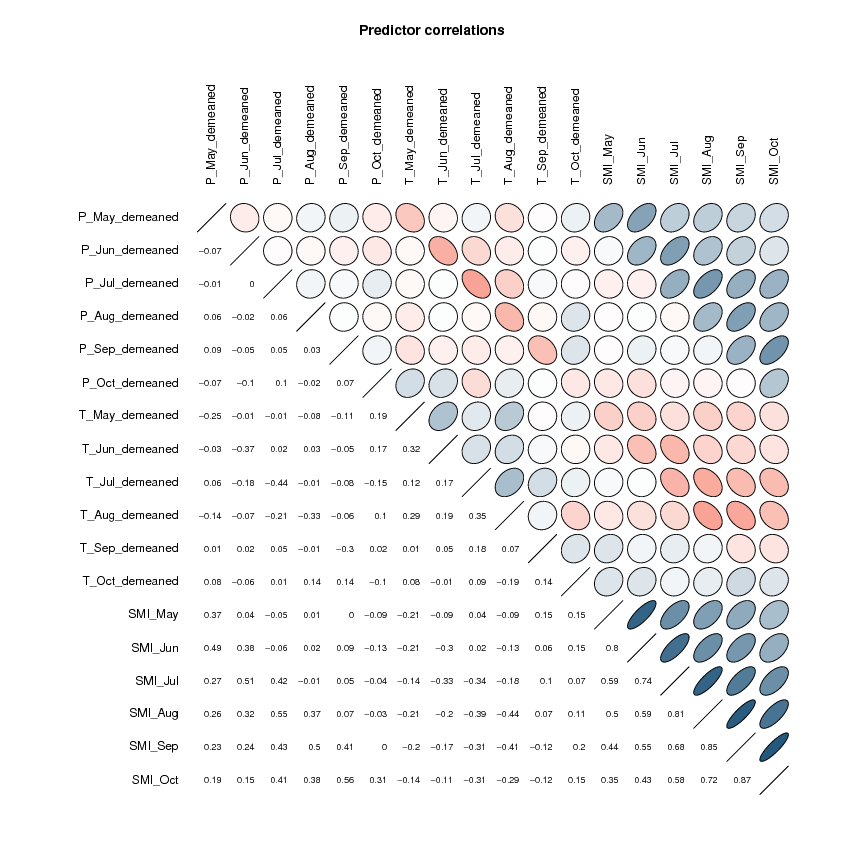
\includegraphics[width=1\textwidth]{PredictorCorrelation.png}
	\caption{Pearson Correlation of the possible predictors used in the model.}
\end{figure}

\subsection{Climate Data}
\section{Methods}
\section{Results}

\section{Discussion}
% \ack
% \appendix 
\newcommand{\newblock}{}
\bibliographystyle{dcu} %{dcu} 
\bibliography{Mendeley.bib}
%\bibliography{high_flows}

\end{document}

%\pacs{00.00, 20.00, 42.10}
% Keywords required only for MST, PB, PMB, PM, JOA, JOB? 
%\vspace{2pc}
%\noindent{\it Keywords}: Article preparation, IOP journals
% Uncomment for Submitted to journal title message
\submitto{\ERL}
% Comment out if separate title page not required
\maketitle


\section{Introduction}
Based on the current research on silage maize sensitivity to monthly weather and soil moisture impacts  a predictive model shall be established.  So far, the goal was to evaluate the causal effects of soil moisture anomalies on a monthly basis. So far, time dependent effects of soil moisture have been evaluated. For instance extreme wetness in the early period and extreme dryness in August are responsible for diminished silage maize yield.  Further, the focus was on in-sample variation. This has methodological implications, as for instance the use of parametric standard errors and the control for confounding factors. Also, it allows to use plm package, which is not so good suited for predictions. 
Now, we derive heuristacially a model which relies on the seasonal effects observed in the paper before. 



\section{Methods}
\subsection{Training Data and Model Fitting}
% Generell denke ich, dass hier der Methodenteil wesentlich kürzer gehalten werden kann als  in Paper 1. 
\subsubsection{(Training Data)}
Test
\subsection{Climate Data}

\section{Results and Discussion}

% \ack
% \appendix 
\newcommand{\newblock}{}
\bibliographystyle{dcu} %{dcu} 
\bibliography{Mendeley.bib}
%\bibliography{high_flows}

\end{document}
